\mychapter{Resultados}
\label{Cap:Resultados}

A plataforma \textbf{DDR} foi desenvolvida para reconciliar dados industriais de forma eficaz, corrigindo inconsistências e aumentando a precisão dos processos produtivos. Utilizando as tecnologias \textit{React.js}, \textit{Python} e \textit{ReactFlow}, a interface da plataforma se mostrou escalável e interativa, adequada para o monitoramento em tempo real de grandes volumes de dados.

A Figura \ref{fig:ReactFlowPicture} ilustra o resultado final da interface do cliente, que oferece uma visualização clara dos fluxos de dados industriais.

\begin{figure}[htbp!]
    \begin{center}
        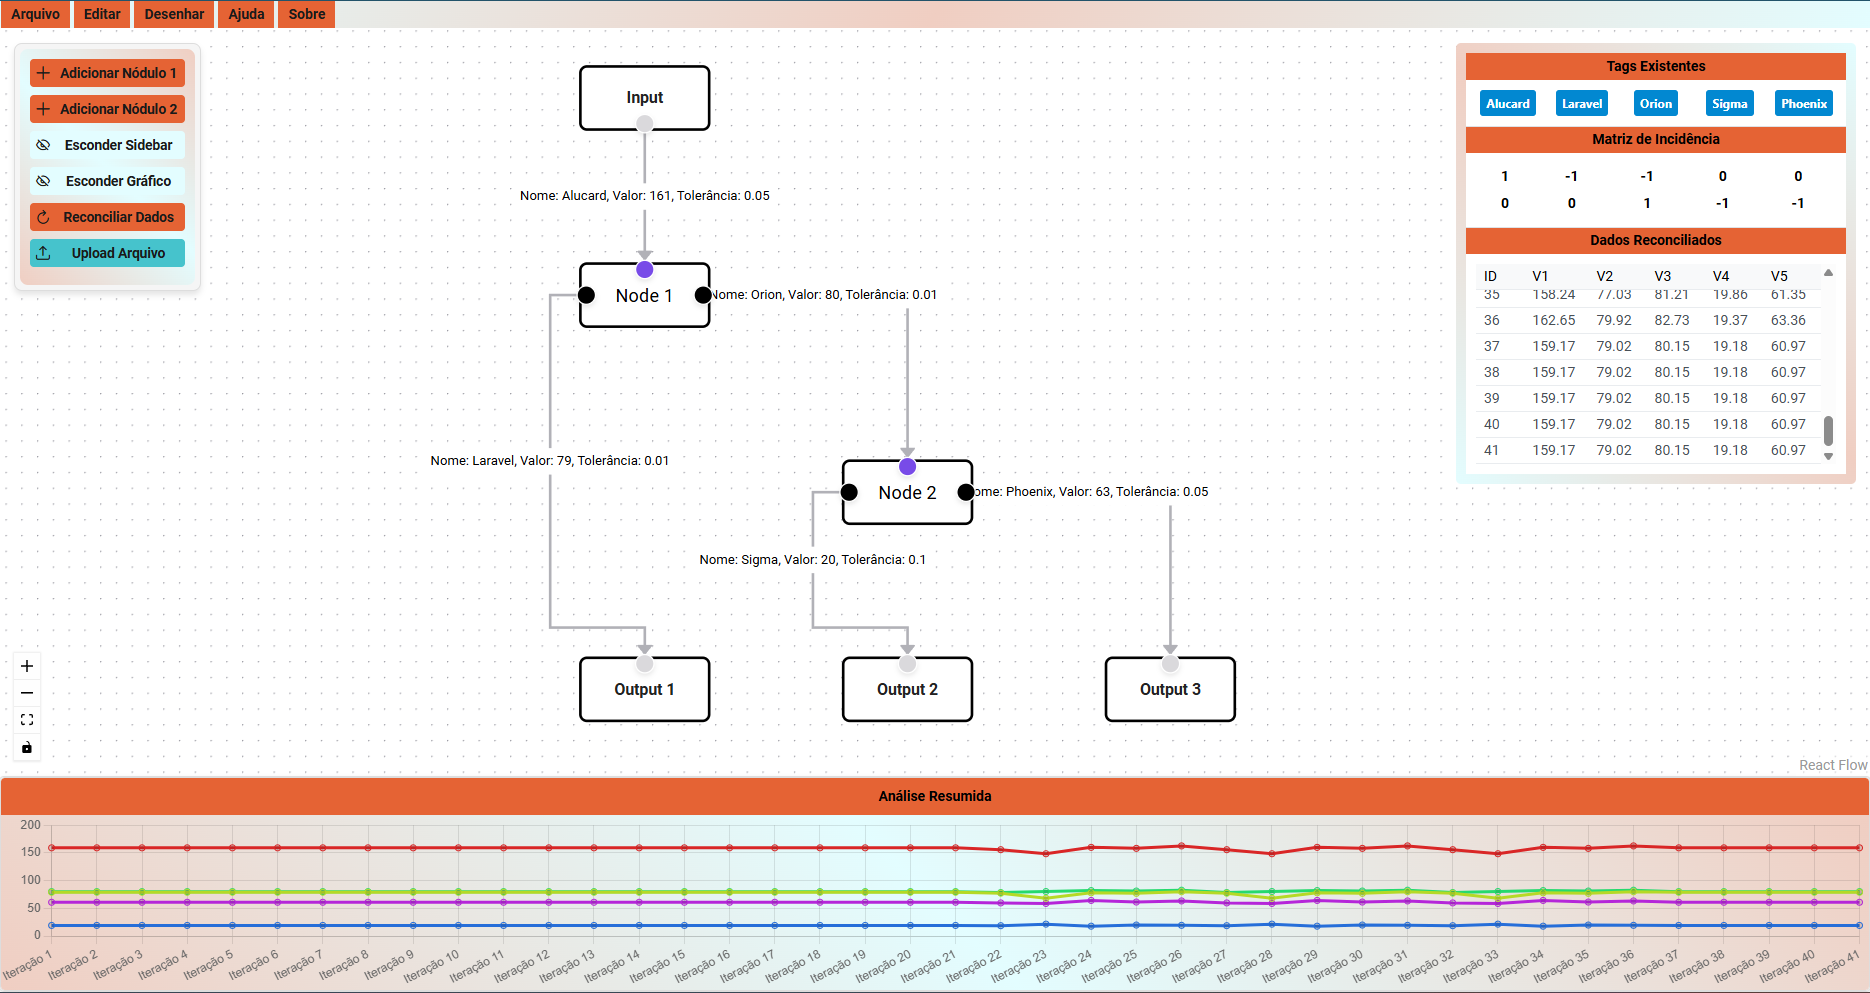
\includegraphics[width=0.75\textwidth]{figuras/principal.png}
        \caption{Interface final do cliente DDR.}
        \label{fig:ReactFlowPicture}
    \end{center}
\end{figure}

O sistema demonstrou excelente desempenho no processamento de grandes volumes de dados, utilizando as bibliotecas \textbf{NumPy} e \textbf{SciPy} para realizar cálculos complexos. O banco de dados \textbf{PostgreSQL} foi responsável por garantir a integridade dos dados e a eficiência nas consultas e operações, mesmo em cenários de alta demanda.

A reconciliação de dados em bateladas foi completamente implementada, corrigindo dados de sensores com base em leis de conservação de massa e energia. O sistema se mostrou eficaz em ajustar os dados brutos, eliminando erros e fornecendo informações consistentes para otimização de processos industriais.

